\documentclass[../main.tex]{subfiles}
\graphicspath{{\subfix{../Images/}}}

\begin{document}

\chapter{Chapter 6. Animation}

This chapter describes various ways to animate objects using Cg. It has the following five sections:

\begin{enumerate}
\item \textbf{"Movement in Time"} introduces the concept of animation.
\item \textbf{"A Pulsating Object"} shows a vertex program that periodically displaces an object's surface outward, in the direction of its normal vectors.
\item \textbf{"Particle Systems"} describes how to use a physically based simulation to create a particle system, with all the calculations done by the GPU.
\item \textbf{"Key-Frame Interpolation"} explains key-frame animation, in which a vertex program animates an object by interpolating between different object poses.
\item \textbf{"Vertex Skinning"} explains how to displace vertices based on multiple weighted control matrices for more dynamic control in character animation.
\end{enumerate}

\section{6.1 Movement in Time}

Animation is the result of an action that happens over time—for example, an object that pulsates, a light that fades, or a character that runs. Your application can create these types of animation using vertex programs written in Cg. The source of the animation is one or more program parameters that vary with the passing of time in your application.

To create animated rendering, your application must keep track of time at a level above Cg and even above OpenGL or Direct3D. Applications typically represent time with a global variable that is regularly incremented as your application's sense of time advances. Applications then update other variables as a function of time.

You could compute animation updates on the CPU and pass the animated data to the GPU. However, a more efficient approach is to perform as much of the animation computation as possible on the GPU with a vertex program, rather than require the CPU to do all the number-crunching. Offloading animation work from the CPU can help balance the CPU and GPU resources and free up the CPU for more involved computations, such as collision detection, artificial intelligence, and game play.

\section{6.2 A Pulsating Object}

In this first example, you will learn how to make an object deform periodically so that it appears to bulge. The goal is to take a time parameter as input and then modify the vertex positions of the object geometry based on the time. More specifically, you need to displace the surface position in the direction of the surface normal, as shown in Figure \ref{fig:6-1}.

\begin{figure}
    \centering
    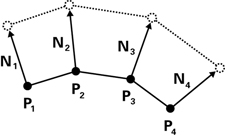
\includegraphics[width=0.5\linewidth]{fig6_1.jpg}
    \caption{Figure 6-1 Making an Object Bulge}
    \label{fig:6-1}
\end{figure}

By varying the magnitude of the displacement over time, you create a bulging or pulsing effect. Figure \ref{fig:6-2} shows renderings of this effect as it is applied to a character. The pulsating animation takes place within a vertex program.

\begin{figure}
    \centering
    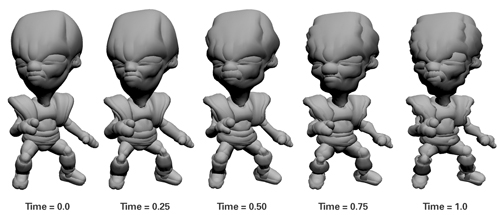
\includegraphics[width=1\linewidth]{fig6_2.jpg}
    \caption{Figure 6-2 A Pulsating Alien}
    \label{fig:6-2}
\end{figure}

\subsection{6.2.1 The Vertex Program}

Example 6-1 shows the complete source code for the \textbf{C6E1v_bulge} vertex program, which is intended to be used with the \textbf{C2E2f_passthrough} fragment program from Chapter 2. Only the vertex position and normal are really needed for the bulging effect. However, lighting makes the effect look more interesting, so we have included material and light information as well. A helper function called \textbf{computeLighting} calculates just the diffuse and specular lighting (the specular material is assumed to be white for simplicity).

\FloatBarrier
\begin{lstlisting}[caption=Example 6-1. The \textbf{C6E1v_bulge} Vertex Program]
float3 computeLighting(float3 lightPosition,
                       float3 lightColor,
                       float3 Kd,
                       float  shininess,
                       float3 P,
                       float3 N,
                       float3 eyePosition)
{
  // Compute the diffuse lighting
  float3 L = normalize(lightPosition - P);
  float diffuseLight = max(dot(N, L), 0);
  float3 diffuseResult = Kd * lightColor * diffuseLight;

  // Compute the specular lighting
  float3 V = normalize(eyePosition - P);
  float3 H = normalize(L + V);
  float3 specularLight = lightColor * pow(max(dot(N, H), 0),
                                          shininess);
  if (diffuseLight <= 0) specularLight = 0;
  float3 specularResult = lightColor * specularLight;
  return diffuseResult + specularResult;
}

void C6E1v_bulge(float4 position  : POSITION,
                 float3 normal    : NORMAL,

             out float4 oPosition : POSITION,
             out float4 color     : COLOR,

         uniform float4x4 modelViewProj,
         uniform float    time,
         uniform float    frequency,
         uniform float    scaleFactor,
         uniform float3   Kd,
         uniform float    shininess,
         uniform float3   eyePosition,
         uniform float3   lightPosition,
         uniform float3   lightColor)
{
  float displacement = scaleFactor * 0.5 *
                       sin(position.y * frequency * time) + 1;
  float4 displacementDirection = float4(normal.x, normal.y,
                                        normal.z, 0);
  float4 newPosition = position +
                       displacement * displacementDirection;
  oPosition = mul(modelViewProj, newPosition);
  color.xyz = computeLighting(lightPosition, lightColor,
                          Kd, shininess,
                          newPosition.xyz, normal,
                          eyePosition);
  color.w = 1;
}
\end{lstlisting}
\FloatBarrier

\subsection{6.2.2 Displacement Calculation}

\subsection*{Creating a Time-Based Function}

The idea here is to calculate a quantity called \textbf{displacement} that moves the vertex position up or down in the direction of the surface normal. To animate the program's effect, \textbf{displacement} has to change over time. You can choose any function you like for this. For example, you could pick something like this:

\FloatBarrier
\begin{lstlisting}
float displacement = time;
\end{lstlisting}
\FloatBarrier

Of course, this behavior doesn't make a lot of sense, because \textbf{displacement} would always increase, causing the object to get larger and larger endlessly over time. Instead, we want a pulsating effect in which the object oscillates between bulging larger and returning to its normal shape. The sine function provides such a smoothly oscillating behavior.

A useful property of the sine function is that its result is always between –1 and 1. In some cases, such as in this example, you don't want any negative numbers, so you can scale and bias the results into a more convenient range, such as from 0 to 1:

\FloatBarrier
\begin{lstlisting}
float displacement = 0.5 * (sin(time) + 1);
\end{lstlisting}
\FloatBarrier

\subsection*{Performance Tip}

Did you know that the \textbf{sin} function is just as efficient as addition or multiplication in the CineFX architecture? In fact, the \textbf{cos} function, which calculates the cosine function, is equally fast. Take advantage of these features to add visual complexity to your programs without slowing down their execution.
\hrule

\subsection*{Adding Controls to the Program}

To allow finer control of your program, you can add a uniform parameter that controls the frequency of the sine wave. Folding this uniform parameter, \textbf{frequency}, into the displacement equation gives:

\FloatBarrier
\begin{lstlisting}
float displacement = 0.5 * (sin(frequency * time) + 1);
\end{lstlisting}
\FloatBarrier

You may also want to control the amplitude of the bulging, so it's useful to have a uniform parameter for that as well. Throwing that factor into the mix, here's what we get:

\FloatBarrier
\begin{lstlisting}
float displacement = scaleFactor * 0.5 *
                     (sin(frequency * time) + 1);
\end{lstlisting}
\FloatBarrier

As it is now, this equation produces the same amount of protrusion all over the model. You might use it to show a character catching his breath after a long chase. To do this, you would apply the program to the character's chest. Alternatively, you could provide additional uniform parameters to indicate how rapidly the character is breathing, so that over time, the breathing could return to normal. These animation effects are inexpensive to implement in a game, and they help to immerse players in the game's universe.

\subsection*{Varying the Magnitude of Bulging}

But what if you want the magnitude of bulging to vary at different locations on the model? To do this, you have to add a dependency on a per-vertex varying parameter. One idea might be to pass in \textbf{scaleFactor} as a varying parameter, rather than as a uniform parameter. Here we show you an even easier way to add some variation to the pulsing, based on the vertex position:

\FloatBarrier
\begin{lstlisting}
float displacement = scaleFactor * 0.5 *
                     sin(position.y * frequency * time) + 1;
\end{lstlisting}
\FloatBarrier

This code uses the \textit{y} coordinate of the position to vary the bulging, but you could use a combination of coordinates, if you prefer. It all depends on the type of effect you are after.

\subsection*{Updating the Vertex Position}

In our example, the displacement scales the object-space surface normal. Then, by adding the result to the object-space vertex position, you get a displaced object-space vertex position:

\FloatBarrier
\begin{lstlisting}
   float4 displacementDirection = float4(normal.x, normal.y,
                                         normal.z, 0);
   float4 newPosition = position +
                        displacement * displacementDirection;
\end{lstlisting}
\FloatBarrier

\subsection*{Precompute Uniform Parameters When Possible}

The preceding example demonstrates an important point. Take another look at this line of code from Example 6-1:

\FloatBarrier
\begin{lstlisting}
   float displacement = scaleFactor * 0.5 *
                        sin(position.y * frequency * time) + 1;
\end{lstlisting}
\FloatBarrier

If you were to use this equation for the displacement, all the terms would be the same for each vertex, because they all depend only on uniform parameters. This means that you would be computing this displacement on the GPU for \textit{each vertex}, when in fact you could simply calculate the displacement on the CPU just once for the entire mesh and pass the displacement as a uniform parameter. However, when the vertex position is part of the displacement equation, the sine function must be evaluated for each vertex. And as you might expect, if the value of the displacement varies for every vertex like this, such a per-vertex computation can be performed far more efficiently on the GPU than on the CPU.

\subsection*{Coding Tip}

If a computed value is a constant value for an entire object, optimize your program by precomputing that value on a per-object basis with the CPU. Then pass the precomputed value to your Cg program as a uniform parameter. This approach is more efficient than recomputing the value for every fragment or vertex processed.
\hrule

\section{6.3 Particle Systems}

Sometimes, instead of animating vertices in a mesh, you want to treat each vertex as a small object, or \textit{particle}. A collection of particles that behave according to specific rules is known as a particle system. This example implements a simple particle system in a vertex program. For now, focus on how the system works; don't worry about its simplistic appearance. At the end of this section, we will mention one easy method to enhance your particle system's appearance. Figure \ref{fig:6-3} shows the particle system example progressing in time.

\begin{figure}
    \centering
    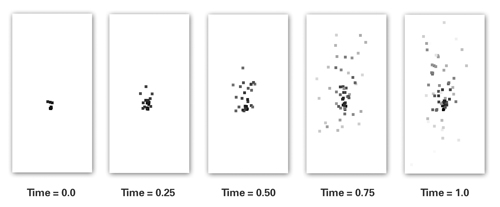
\includegraphics[width=1\linewidth]{fig6_3.jpg}
    \caption{Figure 6-3 A Particle System}
    \label{fig:6-3}
\end{figure}

The example particle system behaves according to a simple vector kinematic equation from physics. The equation gives the \textit{x}, \textit{y}, and \textit{z} positions of each particle for any time. The basic equation from which you will start is shown in Equation 6-1.

\FloatBarrier
\begin{equationcaption}
$
p_{final} = p_{initial} + vt + \frac{1}{2}at^2
$
\caption{Equation 6-1 Particle Trajectory}
\end{equationcaption}
\FloatBarrier

where:

\begin{itemize}
\item $p_{final}$ is the particle's final position,
\item $p_{initial}$ is the particle's initial position,
\item $v$ is the particle's initial velocity,
\item $a$ is the particle's acceleration, and
\item $t$ is the time taken.
\end{itemize}

The equation models the trajectory of a particle set in initial motion and under the influence of gravity, but not otherwise interacting with other particles. This equation gives the position of a particle for any value of time, assuming that you provide its initial position, initial velocity, and constant acceleration, such as gravity.

\subsection{6.3.1 Initial Conditions}

The application must supply the initial position and initial velocity of each particle as varying parameters. These two parameter values are known as \textit{initial conditions} because they describe the particle at the beginning of the simulation.

In this particular simulation, the acceleration due to gravity is the same for every particle. Therefore, gravity is a uniform parameter.

To make the simulation more accurate, you could factor in effects such as drag and even spin—we leave that as an exercise for you.

\subsection{6.3.2 Vectorized Computations}

Modern GPUs have powerful vector-processing capabilities, particularly for addition and multiplication; they are well suited for processing vectors with up to four components. Therefore, it is often just as efficient to work with such vector quantities as it is to work with scalar (single-component) quantities.

Equation 6-1 is a vector equation because the initial position, initial velocity, constant acceleration, and computed position are all three-component vectors. By implementing the particle system equation as a vector expression when writing the Cg vertex program, you help the compiler translate your program to a form that executes efficiently on your GPU.

\subsection*{Performance Tip}

Vectorize your calculations whenever possible, to take full advantage of the GPU's powerful vector-processing capabilities.
\hrule

\subsection{6.3.3 The Particle System Parameters}

Table \ref{table:6-1} lists the variables used by the vertex program presented in the next section.

\begin{table}
\centering
\begin{tabular}{ p{2cm} p{1cm} p{6cm} p{3.5cm}  } 

Variable & Type & Description & Source (Type) \\
\hline

\textbf{pInitial} & \textbf{float3} & Initial position & Application (Varying) \\
\hline
\textbf{vInitial} & \textbf{float3} & Initial velocity & Application (Varying) \\
\hline
\textbf{tInitial} & \textbf{float3} & Time at which particle was created & Application (Varying) \\
\hline
\textbf{acceleration} & \textbf{float3} & Acceleration (0.0, -9.8, 0.0) & Application (Uniform) \\
\hline
\textbf{globalTime} & \textbf{float} & Global time & Application (Uniform) \\
\hline
\textbf{pFinal} & \textbf{float3} & Current position & Internal\\
\hline
\textbf{t} & \textbf{float} & Relative time & Internal \\
\hline

\end{tabular}

\caption{Table 6-1. Variables in the Particle Equation}
\label{table:6-1}
\end{table}

Each variable is a parameter to the vertex program, except for the relative time (\textbf{t}) and final position (\textbf{pFinal}), which are calculated inside the vertex program. Note that the \textit{y} component of the acceleration is negative—because gravity acts downward, in the negative \textit{y} direction. The constant 9.8 meters per second squared is the acceleration of gravity on Earth. The initial position, initial velocity, and uniform acceleration are object-space vectors.

\FloatBarrier
\begin{lstlisting}[caption=Example 6-2. The \textbf{C6E2v_particle} Vertex Program]
void C6E2v_particle(float4 pInitial : POSITION,
                    float4 vInitial : TEXCOORD0,
                    float  tInitial : TEXCOORD1,

                out float4 oPosition : POSITION,
                out float4 color     : COLOR,
                out float  pointSize : PSIZE,

            uniform float    globalTime,
            uniform float4   acceleration,
            uniform float4x4 modelViewProj)
{
  float t = globalTime - tInitial;
  float4 pFinal = pInitial +
                  vInitial * t +
                  0.5 * acceleration * t * t;

  oPosition = mul(modelViewProj, pFinal);

  color = float4(t, t, t, 1);

  pointSize = -8.0 * t * t +
               8.0 * t +
               0.1 * pFinal.y + 1;
}
\end{lstlisting}
\FloatBarrier

\subsection{6.3.4 The Vertex Program}

Example 6-2 shows the source code for the \textbf{C6E2v_particle} vertex program. This program is meant to work in conjunction with the \textbf{C2E2f_passthrough} fragment program.

\subsection*{Computing the Particle Positions}

In this program, the application keeps track of a "global time" and passes it to the vertex program as the uniform parameter \textbf{globalTime}. The global time starts at zero when the application initializes and is continuously incremented. As each particle is created, the particle's time of creation is passed to the vertex program as the varying parameter \textbf{tInitial}. To find out how long a particle has been active, you simply have to subtract \textbf{tInitial} from \textbf{globalTime}:

\FloatBarrier
\begin{lstlisting}
   float t = globalTime - tInitial;
\end{lstlisting}
\FloatBarrier

Now you can plug \textbf{t} into Equation 6-1 to find the particle's current position:

\FloatBarrier
\begin{lstlisting}
   float4 pFinal = pInitial +
                vInitial * t +
                0.5 * acceleration * t * t;
\end{lstlisting}
\FloatBarrier
                
This position is in object space, so it needs to be transformed into clip space, as usual:

\FloatBarrier
\begin{lstlisting}
   oPosition = mul(modelViewProj, pFinal);
\end{lstlisting}
\FloatBarrier

\subsection*{Computing the Particle Color}

In this example, time controls the particle color:

\FloatBarrier
\begin{lstlisting}
   color = float4(t, t, t, 1);
\end{lstlisting}
\FloatBarrier
   
This is a simple idea, but it produces an interesting visual variation. The color increases with time linearly. Note that colors saturate to pure white (1, 1, 1, 1). You can try your own alternatives, such as varying the color based on the particle's position, or varying the color based on a combination of position and time.

\subsection*{Computing the Particle Size}

\textbf{C6E2v_particle} uses a new vertex program output semantic called \textbf{PSIZE}. When you render a point to the screen, an output parameter with this semantic specifies the width (and height) of the point in pixels. This gives your vertex program programmatic control of the point size used by the rasterizer.

The point size of each particle varies as time passes. The particles start out small, increase in size, and then gradually shrink. This variation adds to the fireworks-like effect. As an extra touch, we added a slight dependence on the particles' height, so that they get a little larger on their way up. To accomplish all this, we use the following function for the point size:

\FloatBarrier
\begin{lstlisting}
   pointSize = -8.0 * t * t +
                8.0 * t +
                0.1 * pFinal.y + 1;
\end{lstlisting}
\FloatBarrier
                
Figure \ref{fig:6-4} shows what the function looks like.

\begin{figure}
    \centering
    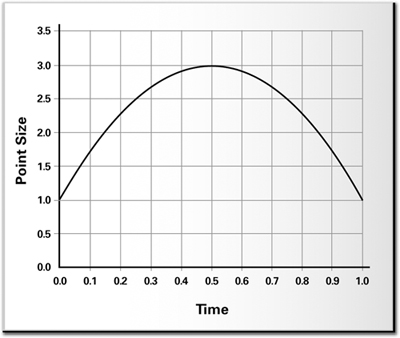
\includegraphics[width=0.75\linewidth]{fig6_4.jpg}
    \caption{Figure 6-4 A Point Size Function}
    \label{fig:6-4}
\end{figure}

This function is nothing special—we merely created the formula to achieve the effect that we wanted. In other words, the formula does not have any real physical meaning, aside from attempting to mimic the effect we had in mind.

\subsection{6.3.5 Dressing Up Your Particle System}

Although the \textbf{C6E2v_particle} program produces interesting particle motion, the particles themselves do not look very appealing—they are just solid-colored squares of different sizes.

However, you can improve the particle appearance by using \textit{point sprites}. With point sprites, the hardware takes each rendered point and, instead of drawing it as a single vertex, draws it as a square made up of four vertices, as shown in Figure \ref{fig:6-5}. Point sprites are automatically assigned texture coordinates for each corner vertex. This allows you to alter the appearance of the particles from a square to any texture image you want.

\begin{figure}
    \centering
    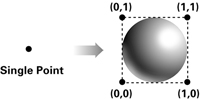
\includegraphics[width=0.5\linewidth]{fig6_5.jpg}
    \caption{Figure 6-5 Converting Points to Point Sprites}
    \label{fig:6-5}
\end{figure}

By rendering the points as point sprites, you can use the assigned texture coordinates to sample a texture that supplies the shape and appearance of each point vertex, instead of simply rendering each point vertex as a square point. Point sprites can create the impression of added geometric complexity without actually drawing extra triangles. Figure \ref{fig:6-6} shows a more visually interesting example of a particle system, using point sprites. Both OpenGL and Direct3D have standard interfaces for rendering point sprites.

\begin{figure}
    \centering
    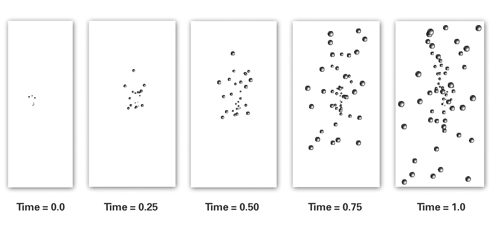
\includegraphics[width=1\linewidth]{fig6_6.jpg}
    \caption{Figure 6-6 A Particle System with Point Sprites}
    \label{fig:6-6}
\end{figure}

\section{6.4 Key-Frame Interpolation}

3D games often use a sequence of key frames to represent an animated human or creature in various poses. For example, a creature may have animation sequences for standing, running, kneeling, ducking, attacking, and dying. Artists call each particular pose that they create for a given 3D model a key frame.

\subsection{6.4.1 Key-Framing Background}

The term \textit{key frame} comes from cartoon animation. To produce a cartoon, an artist first quickly sketches a rough sequence of frames for animating a character. Rather than draw every frame required for the final animation, the artist draws only the important, or "key," frames. Later, the artist goes back and fills in the missing frames. These in-between frames are then easier to draw, because the prior and subsequent key frames serve as before-and-after references.

Computer animators use a similar technique. A 3D artist makes a key frame for each pose of an animated character. Even a standing character may require a sequence of key frames that show the character shifting weight from one foot to the other. Every key frame for a model must use the exact same number of vertices, and every key frame must share the same vertex connectivity. A vertex used in a given key frame corresponds to the same point on the model in every other key frame of the model. The entire animation sequence maintains this correspondence. However, the position of a particular vertex may change from frame to frame, due to the model's animation.

Given such a key-framed model, a game animates the model by picking two key frames and then blending together each corresponding pair of vertex positions. The blend is a weighted average in which the sum of the weights equals 100 percent. Figure \ref{fig:6-7} shows an alien character with several key frames. The figure includes two key frames, marked A and B, to be blended into an intermediate pose by a Cg program.

\begin{figure}
    \centering
    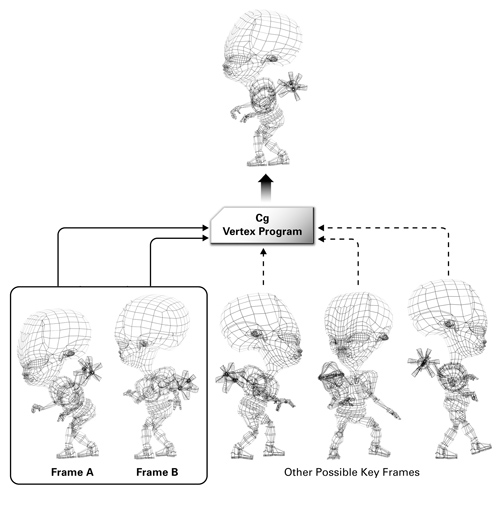
\includegraphics[width=1\linewidth]{fig6_7.jpg}
    \caption{Figure 6-7 Key Frames for an Alien}
    \label{fig:6-7}
\end{figure}

An application can use a Cg vertex program to blend the two vertices together. This blending may include further operations to illuminate the blended character appropriately for more realism. Usually, an application specifies a single position for each vertex, but for key-frame blending, each vertex has two positions, which are combined with a uniform weighting factor.

Key-frame interpolation assumes that the number and order of vertices are the same in all the key frames for a given model. This assumption ensures that the vertex program is always blending the correct pairs of vertices. The following Cg code fragment blends key-frame positions:

\FloatBarrier
\begin{lstlisting}
  blendedPosition = (1 - weight) * keyFrameA + weight * keyFrameB;
\end{lstlisting}
\FloatBarrier

The \textbf{keyFrameA} and \textbf{keyFrameB} variables contain the (\textit{x}, \textit{y}, \textit{z}) positions of the vertex being processed at key frames A and B, respectively. Note that \textbf{weight} and \textbf{(1 – weight)} sum to 1. If weight is 0.53, the Cg program adds 47 percent (1.0 – 0.53) of the position of key frame A to 53 percent of the position of key frame B. Figure \ref{fig:6-8} shows an example of this type of animation.

\begin{figure}
    \centering
    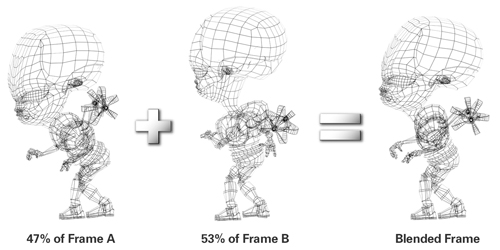
\includegraphics[width=1\linewidth]{fig6_8.jpg}
    \caption{Figure 6-8 An Example of Key-Frame Blending}
    \label{fig:6-8}
\end{figure}

To maintain the appearance of continuous animation, the key-frame weight increases with each rendered frame until it reaches 1.0 (100 percent). At this point, the existing key frame B becomes the new key frame A, the weight resets to 0, and the game selects a new key frame B to continue the animation. Animation sequences, such as walking, may loop repeatedly over the set of key frames that define the character's walking motion. The game can switch from a walking animation to a running animation just by changing over to the sequence of key frames that define the running animation.

It is up to the game engine to use the key frames to generate convincing animated motion. Many existing 3D games use this style of key-frame animation. When an application uses a Cg vertex program to perform the key-frame blending operations, the CPU can spend time improving the gameplay rather than continuously blending key frames. By using a Cg vertex program, the GPU takes over the task of key-frame blending.

\subsection{6.4.2 Interpolation Approaches}

There are many types of interpolation. Two common forms for key-frame interpolation are \textit{linear interpolation} and \textit{quadratic interpolation}.

\subsection*{Linear Interpolation}

With linear interpolation, the transition between positions happens at a constant rate. Equation 6-2 shows the definition of linear interpolation:

\FloatBarrier
\begin{equationcaption}
$
blendedPosition = positionA * (1-f) + positionB * f
$
\caption{Equation 6-2 Linear Interpolation}
\end{equationcaption}
\FloatBarrier

As \textit{f} varies from 0 to 1 in this equation, the intermediate position varies between \textit{positionA} and \textit{positionB}. When \textit{f} is equal to 0, the intermediate position is exactly \textit{positionA}, the starting position. When \textit{f} is equal to 1, the intermediate position is \textit{positionB}, the ending position. Once again, you can use Cg's \textbf{lerp} function to accomplish the interpolation.

Using \textbf{lerp}, the interpolation between two positions can be written concisely as:

\FloatBarrier
\begin{lstlisting}
intermediatePosition = lerp(positionA, positionB, f);
\end{lstlisting}
\FloatBarrier

\subsection*{Quadratic Interpolation}

Linear interpolation is good for many situations, but sometimes you want the rate of transition to change over time. For example, you might want the transition from \textit{positionA} to \textit{positionB} to start out slowly and get faster as time passes. For this, you might use quadratic interpolation, as in the following code fragment:

\FloatBarrier
\begin{lstlisting}
intermediatePosition = position1 * (1 - f * f) +
                       position2 * f * f
\end{lstlisting}
\FloatBarrier

Other functions that you might use are step functions, spline functions, and exponential functions. Figure \ref{fig:6-9} shows several common types of interpolation functions.

\begin{figure}
    \centering
    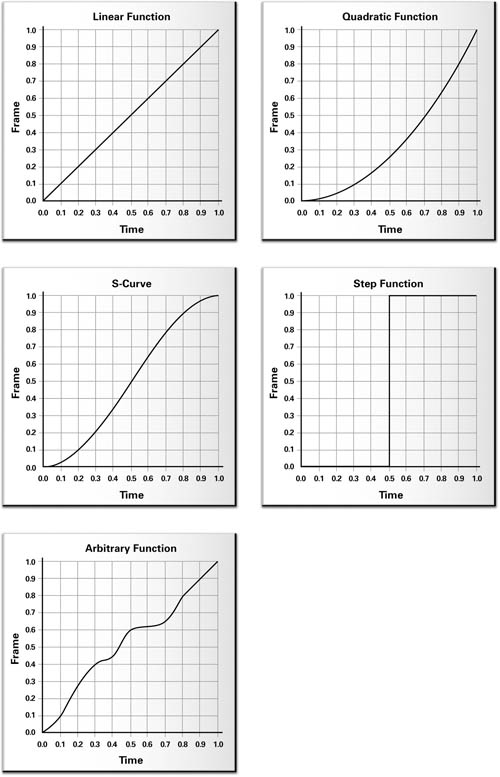
\includegraphics[width=1\linewidth]{fig6_9.jpg}
    \caption{Figure 6-9 Various Interpolation Functions}
    \label{fig:6-9}
\end{figure}

\subsection{6.4.3 Basic Key-Frame Interpolation}

Example 6-3 shows the \textbf{C6E3v_keyFrame} vertex program. This program performs the object-space blending of two positions, each from a different key frame. The \textbf{lerp} Standard Library function linearly interpolates the two positions, and then the program transforms the blended position into clip space. The program passes through a texture coordinate set and a color.

As indicated by the input semantics for \textbf{positionA} and \textbf{positionB}, the application is responsible for configuring key frame A's position as the conventional position (\textbf{POSITION}) and key frame B's position as texture coordinate set 1 (\textbf{TEXCOORD1}).

\FloatBarrier
\begin{lstlisting}[caption=Example 6-3. The \textbf{C6E3v_keyFrame} Vertex Program]
void C6E3v_keyFrame(float3 positionA : POSITION,
                    float3 positionB : TEXCOORD1,
                    float4 color     : COLOR,
                    float2 texCoord  : TEXCOORD0,

                out float4 oPosition : POSITION,
                out float2 oTexCoord : TEXCOORD0,
                out float4 oColor    : COLOR,

            uniform float    keyFrameBlend,
            uniform float4x4 modelViewProj)
{
  float3 position = lerp(positionA, positionB,
                         keyFrameBlend);
  oPosition = mul(modelViewProj, float4(position, 1));
  oTexCoord = texCoord;
  oColor = color;
}
\end{lstlisting}
\FloatBarrier

The application is also responsible for determining the key-frame blending factor via the uniform parameter \textbf{keyFrameBlend}. The value of \textbf{keyFrameBlend} should transition from 0 to 1. Once 1 is reached, the application chooses another key frame in the animation sequence, the old key frame B position input is then configured as the key frame A position input, and the new key-frame position data feeds the key frame B position input.

\subsection{6.4.4 Key-Frame Interpolation with Lighting}

You often want to light a key-framed model. This involves not merely blending two positions (the vertex in two different key frames), but also blending the two corresponding surface normals. Then you can calculate lighting computations with the blended normal. Blending two normals may change the length of the resulting normal, so you must normalize the blended normal prior to lighting.

Example 6-4 shows the \textbf{C6E4v_litKeyFrame} vertex program that adds per-vertex lighting to the \textbf{C6E3v_keyFrame} example. In the updated example, each key frame also supplies its own corresponding per-vertex surface normal.

\FloatBarrier
\begin{lstlisting}[caption=Example 6-4. The \textbf{C6E4v_litKeyFrame} Vertex Program]
struct Light {
  float3 eyePosition;    // In object space
  float3 lightPosition;  // In object space
  float4 lightColor;
  float  specularExponent;
  float  ambient;
};

float4 computeLighting(Light light,
                       float3 position,  // In object space
                       float3 normal)    // In object space
{
  float3 lightDirection = light.lightPosition - position;
  float3 lightDirNorm = normalize(lightDirection);
  float3 eyeDirection = light.eyePosition - position;
  float3 eyeDirNorm = normalize(eyeDirection);
  float3 halfAngle = normalize(lightDirNorm + eyeDirNorm);
  float diffuse = max(0, dot(lightDirNorm, normal));
  float specular = pow(max(0, dot(halfAngle, normal)),
                       light.specularExponent);
  return light.lightColor * (light.ambient +
                             diffuse + specular);
}

void C6E4v_litKeyFrame(float3 positionA : POSITION,
                       float3 normalA   : NORMAL,
                       float3 positionB : TEXCOORD1,
                       float3 normalB   : TEXCOORD2,
                       float2 texCoord  : TEXCOORD0,

                   out float4 oPosition : POSITION,
                   out float2 oTexCoord : TEXCOORD0,
                   out float4 color     : COLOR,

               uniform float     keyFrameBlend,
               uniform Light     light,
               uniform float4x4  modelViewProj)
{
  float3 position = lerp(positionA, positionB,
                         keyFrameBlend);
  float3 blendNormal = lerp(normalA, normalB,
                            keyFrameBlend);
  float3 normal = normalize(blendNormal);
  oPosition = mul(modelViewProj, float4(position, 1));
  oTexCoord = texCoord;
  color = computeLighting(light, position, normal);
}
\end{lstlisting}
\FloatBarrier

The \textbf{computeLighting} internal function computes a conventional lighting model using object-space lighting.

\section{6.5 Vertex Skinning}

Another approach to animating characters is vertex \textit{skinning}. Many 3D modeling packages author 3D content suitable for vertex skinning. The technique is also known as \textit{matrix palette blending}.

\subsection{6.5.1 The Theory of Vertex Skinning}

Rather than have key frames for each pose of a character, vertex skinning maintains a single default pose and a large set of matrices that appropriately rotate and translate various subregions of the default pose's polygonal mesh. For reasons that will become apparent, these various matrix transforms are often called "bones."

One or more of these matrices control each vertex in the default pose's polygonal mesh. Each matrix is assigned a weighting factor (from 0 to 100 percent), which indicates how much that matrix affects each vertex. Only a small number of matrices usually control each vertex, meaning that only these few matrices have positive and significant weighting factors for a given vertex. We call this small set of matrices the \textit{bone set} for each vertex. We assume that the weighting factors for all the matrices in a vertex's bone set always sum to 100 percent.

When rendering this type of model, you first transform every vertex by each matrix in the vertex's bone set, then weight the results of each matrix transform according to the matrix's corresponding weighting factor, and finally sum the results. This new position is the \textit{skinned vertex position}.

When all the matrices are identity matrices (no rotation, no translation), the mesh is in the default pose. 3D artists often pick a default pose in which the character is standing and facing forward, with legs apart and arms outstretched.

\subsection*{Constructing Poses from Matrices}

By controlling the matrices, you can create novel poses. For example, a vertex on a character's forearm close to the elbow might use 67 percent of the forearm matrix, 21 percent of the elbow matrix, and 12 percent of the upper arm matrix. The animator who creates a model for vertex skinning must appropriately localize each matrix so that, for example, the matrix that controls the left shoulder has no effect on vertices near the ankle. Often, the number of matrices affecting any given vertex is limited to no more than four. For the 3D artist, once all the weights and matrices are assigned to the model's default pose, constructing a new pose is a matter of manipulating the matrices appropriately, rather than attempting to position each individual vertex. Posing and animating the model is much simpler when it is authored for vertex skinning.

For a character model, the most significant matrices represent the way rigid bones in the character's body move and rotate; hence, the vertex-skinning matrices are called \textit{bones}. The vertices represent points on the skin. Vertex skinning simulates how bones, represented as matrices, tug and reposition various points, represented as vertices, on the character's skin.

\subsection*{Lighting}

For correct lighting, you can compute the same sort of transformed and weighted average used for positions, except that you transform normals by the inverse transpose of each matrix rather than by the matrix itself. Weighted normals may no longer be unit length, so normalization is required.

Assuming that the bone matrices are merely rotations and translations simplifies the transformation of the normals for lighting, because the inverse transpose of a matrix without scaling or projection is the matrix itself.

\subsection*{Storage Requirements Compared with Key Frames}

With the key frame approach, every pose requires a distinct set of vertex positions and normals. This becomes unwieldy if huge numbers of poses are required.

However, with vertex skinning, each pose requires just the default pose—shared by all poses—and the matrix values for the given pose. There are generally substantially fewer matrices per character than vertices, so representing a pose as a set of bone matrices is more compact than representing the pose with a key frame. With vertex skinning, you can also create novel poses dynamically, either by blending existing bone matrices from different poses or by controlling matrices directly. For example, if you know what matrices control an arm, you can wave the arm by controlling those matrices.

In addition to requiring the matrices for each pose, the model's default pose needs each vertex to have a default position, a default normal, some number of matrix indices to identify which subset of matrices control the vertex, and the same number of weighting factors, corresponding to each respective matrix.

This data for the default pose is constant for all other poses. Generating a new pose requires only new matrices, not any changes to the default pose data. If the GPU can perform all the vertex-skinning computations, this means that the CPU needs to update only the bone matrices for each new pose, but not otherwise manipulate or access the default pose data.

Vertex skinning is quite amenable to storing and replaying motion-capture sequences. You can represent each motion-capture frame as a set of bone matrices that you can then apply to different models that share the same default pose and matrix associations. Inverse kinematics solvers can also generate bone matrices procedurally. An inverse kinematics solver attempts to find an incremental sequence of bone matrices that transition from one given pose to another given pose in a realistic, natural manner.

\subsection{6.5.2 Vertex Skinning in a Vertex Program}

The \textbf{C6E5v_skin4m} vertex program in Example 6-5 implements vertex skinning, assuming that no more than four bone matrices affect each vertex (a common assumption).

An array of 24 bone matrices, each a 3x4 matrix, represents each pose. The entire array is a uniform parameter to the program. The program assumes that each bone matrix consists of a translation and a rotation (no scaling or projection).

The per-vertex \textbf{matrixIndex} input vector provides a set of four bone-matrix indices for accessing the \textbf{boneMatrix} array. The per-vertex \textbf{weight} input vector provides the four weighting factors for each respective bone matrix. The program assumes that the weighting factors for each vertex sum to 100 percent.

\subsection*{Performance Tip}

For performance reasons, the program treats \textbf{boneMatrix} as an array of \textbf{float4} vectors rather than an array of \textbf{float3x4} matrices. The \textbf{matrixIndex} array contains floating-point values instead of integers, and so the addressing of a single array of vectors is more efficient than accessing an array of matrices. The implication of this is that the indices in the \textbf{matrixIndex} vector should be three times the actual matrix index. So, the program assumes 0 is the first matrix in the array, 3 is the second matrix, and so on. The indices are fixed for each vertex, so you improve performance by moving this "multiply by 3" outside the vertex program.
\hrule

A \textbf{for} loop, looping four times, transforms the default pose position and normal by each bone matrix. Each result is weighted and summed.

The program computes both the weighted position and normal for the pose. The same \textbf{computeLighting} internal function from Example 6-4 computes per-vertex object-space lighting with the weighted position and normal.

Although this example is rather limited, you could generalize it to handle more bone matrices, general bone matrices (for example, allowing scaling), and matrices influencing each vertex—and to compute a better lighting model.

\FloatBarrier
\begin{lstlisting}[caption=Example 6-5. The C6E5v_skin4m Vertex Program]

void C6E5v_skin4m(float3 position    : POSITION,
                  float3 normal      : NORMAL,
                  float2 texCoord    : TEXCOORD0,
                  float4 weight      : TEXCOORD1,
                  float4 matrixIndex : TEXCOORD2,

              out float4 oPosition : POSITION,
              out float2 oTexCoord : TEXCOORD0,
              out float4 color     : COLOR,

          uniform Light light,
          uniform float4    boneMatrix[72], // 24 matrices
          uniform float4x4  modelViewProj)
{
  float3 netPosition = 0, netNormal = 0;

  for (int i = 0; i < 4; i++) {
    float index = matrixIndex[i];
    float3x4 model = float3x4(boneMatrix[index + 0],
                              boneMatrix[index + 1],
                              boneMatrix[index + 2]);
    float3 bonePosition = mul(model, float4(position, 1));
    // Assume no scaling in matrix, just rotate & translate
    float3x3 rotate = float3x3(model[0].xyz,
                               model[1].xyz,
                               model[2].xyz);
    float3 boneNormal = mul(rotate, normal);
    netPosition += weight[i] * bonePosition;
    netNormal   += weight[i] * boneNormal;
  }
  netNormal = normalize(netNormal);

  oPosition = mul(modelViewProj, float4(netPosition, 1));
  oTexCoord = texCoord;
  color = computeLighting(light, netPosition, netNormal);
}
\end{lstlisting}
\FloatBarrier

\section{6.6 Exercises}

\begin{itemize}

\item \textbf{Answer this:} What are some common types of interpolation functions for key-frame interpolation? Describe situations in which you might use each one.

\item \textbf{Try this yourself:} Make the bulging program also glow periodically by adding an emissive term that varies with the time. As a further step, base the emissive term at each vertex on the vertex's diffuse material color.

\item \textbf{Try this yourself:} Optimize the \textbf{C6E2v_particle} program by passing \textbf{t}, \textbf{0.5*t*t}, and \textbf{-0.8*t*t+0.8*t} as uniform parameters.

\item \textbf{Try this yourself:} The particle system you implemented used specific functions for the particle size and color. Try replacing these with functions of your own. One interesting idea for the particle size is to make it dependent on the distance from the eye position. To do this, modify the application to pass the eye position as a uniform parameter to the vertex program. You can then compute the distance from any particle to the eye position and scale based on $1/distance^2$ or some similar function that you prefer.

\item \textbf{Try this yourself:} If you vary the twisting angle temporally, the \textbf{C3E4v_twist} example in Chapter 3 becomes a procedural 2D animation. Write a 3D version of animated twisting and apply it to 3D models.

\item \textbf{Try this yourself:} Modify the \textbf{C6E5v_skin4m} example to handle bone matrices that include scaling. Keep in mind that the inverse transpose matrix required for transforming normals is distinct from the matrix required to transform positions if that matrix includes scaling.

\item \textbf{Try this yourself:} Modify the \textbf{C6E5v_skin4m} example to handle six bone matrices per vertex instead of just four. This means that you may need to split the weights and matrix indices into multiple input parameters.
\end{itemize}

\section{6.7 Further Reading}

If you are interested in the physics behind the particle system you created, you can learn more by reviewing kinematics in any high school or college physics textbook.

Jeff Lander wrote a series of articles in 1998 and 1999 for \textit{Game Developer Magazine} about various animation techniques. You can find these articles on the \textbf{www.darwin3d.com} Web site. For particle systems, read "The Ocean Spray in Your Face." For vertex skinning, check out "Skin Them Bones: Game Programming for the Web Generation."

The original volume of \textit{Game Programming Gems} (Charles River Media, 2000), edited by Mark DeLoura, contains several gems related to key-frame animation and vertex skinning. Check out these articles: "Interpolated 3D Keyframe Animation," by Herbert Marselas; "A Fast and Simple Skinning Technique," by Torgeir Hagland; and "Filling the Gaps—Advanced Animation Using Stitching and Skinning," by Ryan Woodland.

John Vince's book \textit{3-D Computer Animation} (Addison-Wesley, 1992) covers many of the techniques described in this chapter, as well as others, such as free-form deformation (FFD).

DirectX 8 added point sprites to Direct3D. OpenGL implementations from multiple hardware vendors support the \textbf{NV_point_sprite} extension. The specification for this OpenGL extension is available at the \textbf{www.opengl.org} Web site.

\end{document}